\chapter{Introduction}
\label{sec:introduction}

Our Galaxy, the Milky Way, is a barred spiral galaxy made up of a central bulge, a dominant
stellar disk and a diffuse stellar halo (Figure~\ref{fig:milky_way}). The Sun sits inside the
disk at a distance of approximately 8~kpc from the Galactic center, about halfway out to its
edge at a radius of roughly 15~kpc \citep{BlandHawthorn2016}. Everything discussed in this
thesis happens within a few hundred parsecs of the Sun, a fraction of its distance to the
Galactic center.

\begin{figure}[h!]
    \centering
    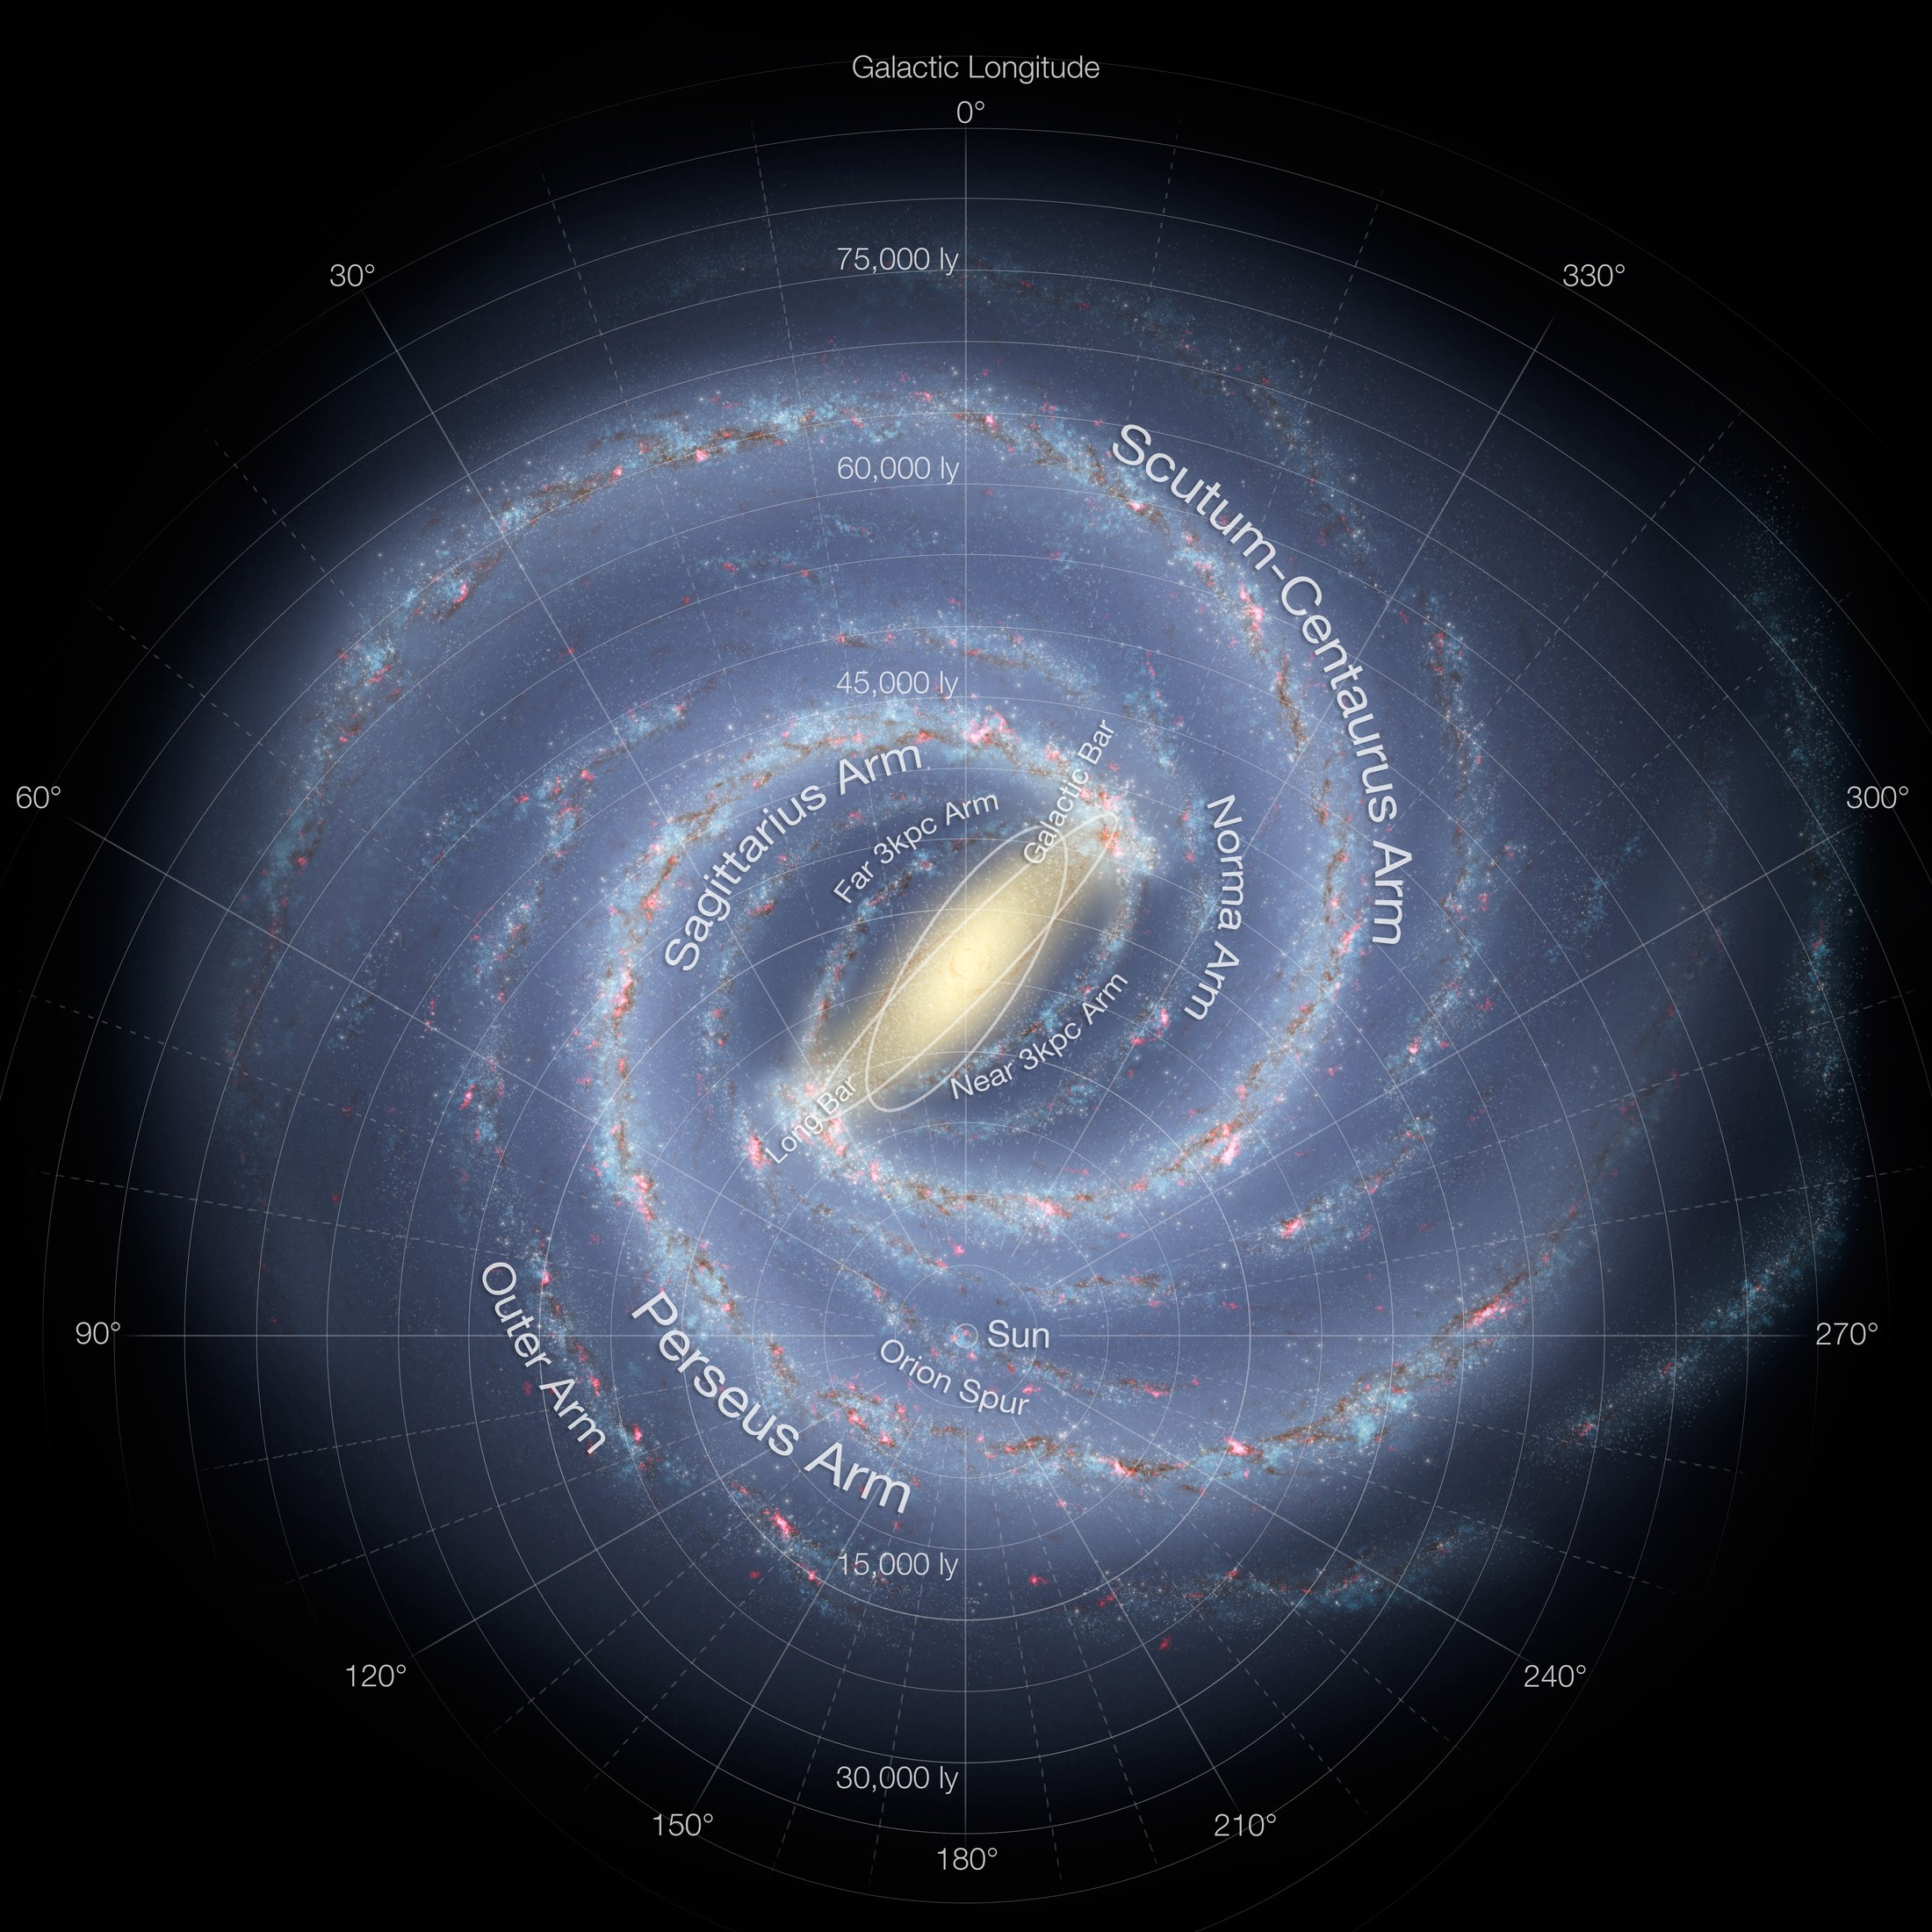
\includegraphics[width=0.75\linewidth]{figures/milky_way.jpg}
    \caption{Artist's impression of the Milky Way seen face-on, with the spiral arms, the central
        bar and the position of the Sun indicated. Rings mark the distance from the Sun in light years,
        radial lines the Galactic longitude. The region studied in this thesis lies within a
        few hundred parsecs of the Sun and is far smaller than any structure labelled here.
        Image credit: \citet{Hurt2013}.}
    \label{fig:milky_way}
\end{figure}

Within this patch, the Sun lies close to the center of a large cavity of hot, low-density gas
that is bounded by a shell of cold gas and dust with a present-day radius of about $165$~pc:
the Local Bubble \citep{Zucker2022}. Almost all young star-forming regions near the Sun are
found on the surface of this shell rather than inside the cavity, a connection that makes the
local neighborhood a valuable laboratory for studying supernova-driven star formation.

One of these regions on the surface of the Local Bubble is the Taurus molecular cloud (TMC),
which is the subject of this thesis. Taurus is one of the most intensively studied star-forming
regions in the Milky Way. Its close proximity to the Sun allows young stellar objects~(YSOs)
to be spatially resolved and characterized individually across the full complex. Unlike
denser, high-mass regions such as the Orion Nebula Cluster, Taurus is an example of
low-density star formation \citep{Luhman2018}, making it possible to study the formation
of solar-type stars in relative isolation. Its stellar population spans the full range of
early evolutionary stages, from deeply embedded protostars to more evolved, disk-free
pre-main-sequence stars \citep{Luhman2023}.

The aim of this thesis is to study the kinematics of the Taurus star-forming region. So far,
this has mainly been done by looking at the discrete, scattered velocities of individual stars.
However, a full 3D space velocity can only be obtained for stars that also have a measured
radial velocity, which is not the case for every member of the complex (only about one third),
so for many stars only the two-dimensional proper motion is known. Discarding those stars would
mean setting aside two thirds of the sample, so this thesis instead seeks a clearer picture by inferring a three-dimensional
velocity field from all the available stellar velocity data. This velocity field is reconstructed using Numerical
Information Field Theory (NIFTy), a Bayesian framework for field inference that models
the continuous velocity field on a three-dimensional grid. The input data consist of three-dimensional
positions, proper motions and, where available, radial velocities all from the latest
Gaia~DR3 measurements \citep{GaiaCollaboration2023}. The resulting velocity field allows further analysis
of both the motion of the whole Taurus complex and the internal kinematics of its substructures.

The thesis is structured as follows: Chapter~\ref{sec:Taurus} gives a short introduction
to already present knowledge about the TMC and its kinematics. Chapter~\ref{sec:Methods}
briefly explains the methods used to reconstruct a continuous field out of the velocity
data. Chapter~\ref{sec:Results} presents the resulting 3D velocity field and discusses possible
findings and caveats of the result, before Chapter~\ref{sec:Conclusion} summarizes them.